%% functional_annotation.tex
%% Author: Leighton Pritchard
%% Copyright: James Hutton Institute
%% A brief description of functional annotation

% SUBSECTION: Functional Annotation
\subsection{Functional Annotation}

% Principles of function prediction
\begin{frame}
  \frametitle{Principles of function prediction}
  At genome scale, we realistically have to automate function prediction. \\
  Function prediction is just like any other prediction method. \\
  Two main approaches to function prediction:
  \begin{itemize}
    \item \textit{ab initio} prediction (on basis of feature sequence/context only)
    \begin{itemize}
      \item Unsupervised methods - not trained on an exemplar dataset
      \item Supervised methods - trained on an exemplar dataset
    \end{itemize}
    \item homology matches (sequence similarity)
    \begin{itemize}
      \item alignment to features with known/predicted functions
    \end{itemize}
  \end{itemize}
\end{frame}

% Homology-based methods
\begin{frame}
  \frametitle{Homology-based function prediction}
  Two proteins with similar sequence may have similar function.\\
  But$\ldots$
  \begin{itemize}
    \item How similar do they have to be (and where) to share the same function?
    \item What do we mean by `same function': interaction/substrate specificity? participation in a pathway? contribution to a structure? biochemical interconversion? $\ldots$
    \item How confident can we be in the comparator (annotated) sequence: was \textit{that} function determined experimentally?
  \end{itemize}
\end{frame}

% Gene Ontology
\begin{frame}
  \frametitle{Gene Ontology (GO)\footnote{\tiny{\href{http://dx.doi.org/10.1038/75556}{Ashburner \textit{et al}. (2000) \textit{Nat. Genet.} \textbf{25}:25-29 doi:10.1038/75556}}}}
  The Gene Ontology provides a common vocabulary for describing biological function, and unifying functional descriptions.\\[0.1cm]
  Gene Ontology Consortium: \href{http://geneontology.org/}{http://geneontology.org/} \\[0.1cm]
  Many annotation tools and databases produce GO output, or compatible controlled vocabulary terms, e.g.
  \begin{itemize}
    \item Blast2GO\footnote{\tiny{\href{http://dx.doi.org/10.1093/bioinformatics/bti610}{Conesa \textit{et al}. (2005) \textit{Bioinformatics} \textbf{21}:3674-3676 doi:10.1093/bioinformatics/bti610}}}: BLAST-based annotation
    \item PHI-Base\footnote{\tiny{\href{http://dx.doi.org/10.1093/nar/gkj047}{Winnenburg \textit{et al}. (2006) \textit{Nuc. Acids Res.} \textbf{34}:D459-D464 doi:10.1093/nar/gkj047}}}: microbial pathogen-host interaction specific functions
    \item GOPred\footnote{\tiny{\href{http://dx.doi.org/10.1371/journal.pone.0012382}{Sarac \textit{et al}. (2010) \textit{PLoS One} \textbf{5}:e12382 doi:10.1371/journal.pone.0012382}}}: combines several protein function classifiers
  \end{itemize}
\end{frame}

% How good are database annotations?
\begin{frame}
  \frametitle{How good are database annotations?\footnote{\tiny{\href{http://dx.doi.org/10.1371/journal.pcbi.1003063}{Schnoes \textit{et al}. (2013) \textit{PLoS Comp. Biol.} \textbf{9}:e1003063 doi:10.1371/journal.pcbi.1003063}}}}
  Are protein functions in databases determined experimentally, or by annotation transfer?\\[0.1cm]
  High throughput experiments and genome annotations conducted without validation of function, and placed in databases.\\[0.1cm]
  \begin{itemize}
    \item GO databases record annotation origin by publication 
    \item GO databases record evidence codes, e.g.: \textbf{EXP}=Inferred from Experiment; \textbf{ISS}=Inferred from Sequence Similarity
    \item 0.14\% of contributing publications provide 25\% of all experimentally validated annotations in the Uniprot-GOA compilation.
    \item There are biases in functional annotation.
  \end{itemize}
  No clear solution to this kind of bias - \textbf{but we have to recognise and account for it}.
\end{frame}

% How good are database annotations?
\begin{frame}
  \frametitle{How good are database annotations?\footnote{\tiny{\href{http://dx.doi.org/10.1038/nmeth.2340}{Radivojac \textit{et al}. (2013) \textit{Nat. Meth.} \textbf{10}:221-227 doi:10.1038/nmeth.2340}}}}
  The Critical Assessment of Function Annotation (CAFA) project.
  \begin{center}
    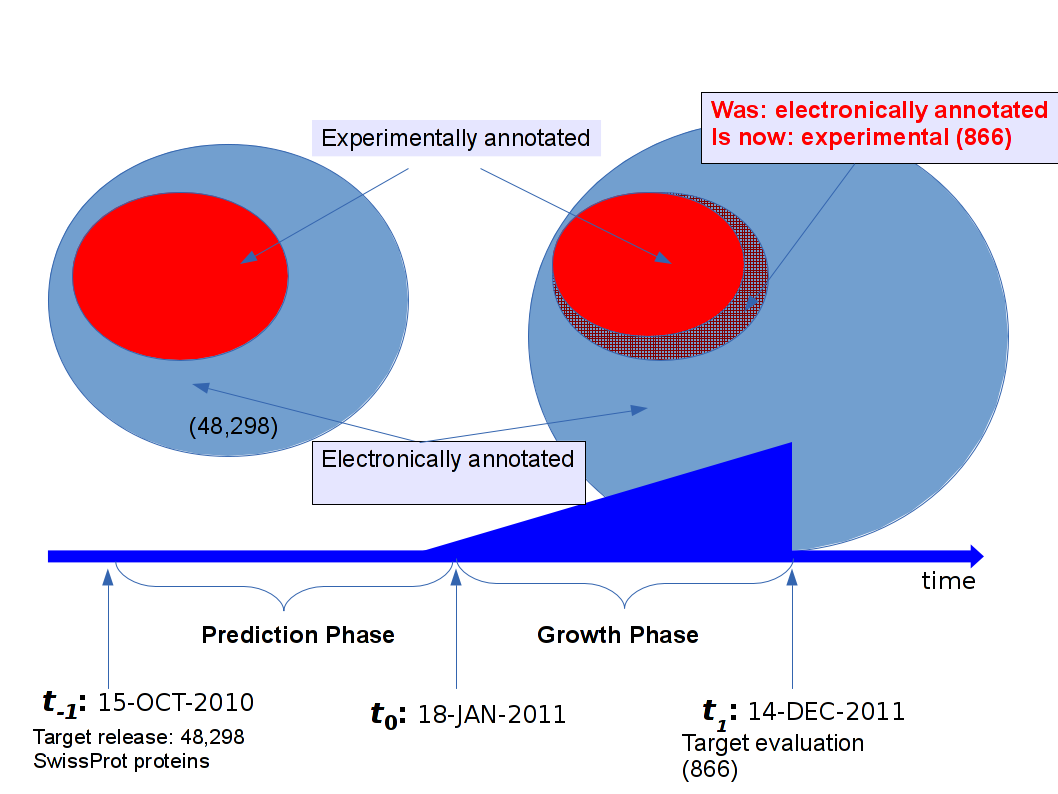
\includegraphics[height=0.7\textheight]{images/cafa_annotation_problem}
  \end{center}   
\end{frame}

% Homology-based methods
\begin{frame}
  \frametitle{Do biased database annotations matter?}
  Experimental annotations of proteins are incomplete. But is that important?\\
  Tested by simulation, and following databases for three years.\footnote{\tiny{\href{http://dx.doi.org/10.1093/bioinformatics/btu472}{Jiang \textit{et al}. (2014) \textit{Bioinformatics} \textbf{30}:i609-i616 doi:10.1093/bioinformatics/btu472}}}
  \begin{enumerate}
    \item Yes. It matters.
    \item Current large scale evaluations are meaningful and almost surprisingly reliable.
    \item The nature and level of data incompleteness, and type of classification model have an effect.
    \item ``Low precision, high recall'' (i.e. less discriminating) tools most significantly affected.
  \end{enumerate}
  Molecular function prediction is usually more reliable than biological process prediction\footnote{\tiny{\href{http://dx.doi.org/10.1186/1471-2105-14-S3-S1}{Cozzetto \textit{et al}. (2013) \textit{BMC Bioinf.} \textbf{14}:S3-S1 doi:10.1186/1471-2105-14-S3-S1}}}
\end{frame}

% How good are database annotations?
\begin{frame}
  \frametitle{CAFA results\footnote{\tiny{\href{http://dx.doi.org/10.1038/nmeth.2340}{Radivojac \textit{et al}. (2013) \textit{Nat. Meth.} \textbf{10}:221-227 doi:10.1038/nmeth.2340}}}}
  The Critical Assessment of Function Annotation (CAFA) 2013 results. {\tiny(F-measure combines precision and recall)}
  \begin{columns}[T]
    \begin{column}{5cm}  
      \begin{itemize}  
        \item You \textbf{can} do better than BLAST.
        \item Once you do better than BLAST, there's not much between methods.
        \item Best methods used evolutionary relationships, structure, and expression data.
        \item Machine Learning works best.
      \end{itemize}
    \end{column}
    \begin{column}{5cm}      
      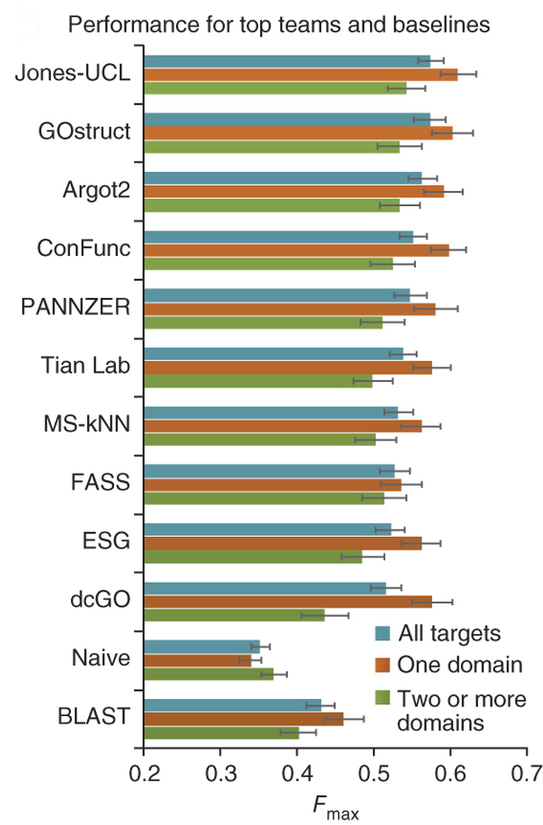
\includegraphics[height=0.65\textheight]{images/cafa_results}
    \end{column}
  \end{columns}         
\end{frame}